% Fig. 1 teaser: full-width, set under the title by main.tex (\twocolumn[{...}]).
% Selected three-column draft (2026-11-03): figures/Fig1/INDEX.md.
\begin{center}
\captionsetup{type=figure}
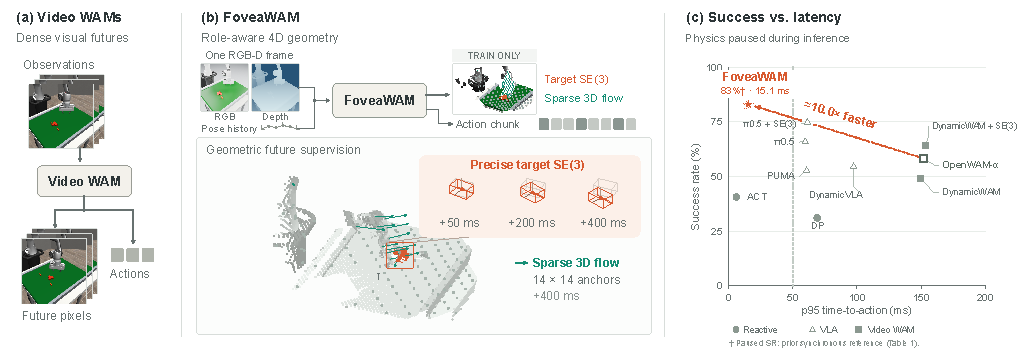
\includegraphics[width=\textwidth]{figures/Fig1/fig1.pdf}
\captionof{figure}{\textbf{\ours allocates prediction precision by task role.}
(a) Reference recordings illustrate dense video-future prediction and action outputs.
(b) One RGB-D frame and pose history condition \ours. Target SE(3) and sparse 3D flow
provide training-only supervision; action chunks are produced at deployment.
The cropped point cloud shows current reference geometry, while future poses and flow
are ground-truth supervision, not model predictions. Flow is sampled on a
\cfgContextGrid{} grid; arrows show 400\,ms displacements enlarged $3\times$.
Pose glyphs show the target at $+50$, $+200$, and $+400$\,ms.
(c) Table~\ref{tab:main} Paused success (physics paused during inference) versus native
p95 time-to-action. The dashed line marks 50\,ms. The \ours star (83\%, 28\,ms) and
the resulting $\approx5.4\times$ speedup over OpenWAM-$\alpha$ (151.7\,ms) are
provisional layout values pending measurement.}
\label{fig:teaser}
\end{center}
